% Options for packages loaded elsewhere
\PassOptionsToPackage{unicode}{hyperref}
\PassOptionsToPackage{hyphens}{url}
\PassOptionsToPackage{dvipsnames,svgnames,x11names}{xcolor}
%
\documentclass[
  letterpaper,
  DIV=11,
  numbers=noendperiod]{scrartcl}

\usepackage{amsmath,amssymb}
\usepackage{iftex}
\ifPDFTeX
  \usepackage[T1]{fontenc}
  \usepackage[utf8]{inputenc}
  \usepackage{textcomp} % provide euro and other symbols
\else % if luatex or xetex
  \usepackage{unicode-math}
  \defaultfontfeatures{Scale=MatchLowercase}
  \defaultfontfeatures[\rmfamily]{Ligatures=TeX,Scale=1}
\fi
\usepackage{lmodern}
\ifPDFTeX\else  
    % xetex/luatex font selection
\fi
% Use upquote if available, for straight quotes in verbatim environments
\IfFileExists{upquote.sty}{\usepackage{upquote}}{}
\IfFileExists{microtype.sty}{% use microtype if available
  \usepackage[]{microtype}
  \UseMicrotypeSet[protrusion]{basicmath} % disable protrusion for tt fonts
}{}
\makeatletter
\@ifundefined{KOMAClassName}{% if non-KOMA class
  \IfFileExists{parskip.sty}{%
    \usepackage{parskip}
  }{% else
    \setlength{\parindent}{0pt}
    \setlength{\parskip}{6pt plus 2pt minus 1pt}}
}{% if KOMA class
  \KOMAoptions{parskip=half}}
\makeatother
\usepackage{xcolor}
\setlength{\emergencystretch}{3em} % prevent overfull lines
\setcounter{secnumdepth}{5}
% Make \paragraph and \subparagraph free-standing
\makeatletter
\ifx\paragraph\undefined\else
  \let\oldparagraph\paragraph
  \renewcommand{\paragraph}{
    \@ifstar
      \xxxParagraphStar
      \xxxParagraphNoStar
  }
  \newcommand{\xxxParagraphStar}[1]{\oldparagraph*{#1}\mbox{}}
  \newcommand{\xxxParagraphNoStar}[1]{\oldparagraph{#1}\mbox{}}
\fi
\ifx\subparagraph\undefined\else
  \let\oldsubparagraph\subparagraph
  \renewcommand{\subparagraph}{
    \@ifstar
      \xxxSubParagraphStar
      \xxxSubParagraphNoStar
  }
  \newcommand{\xxxSubParagraphStar}[1]{\oldsubparagraph*{#1}\mbox{}}
  \newcommand{\xxxSubParagraphNoStar}[1]{\oldsubparagraph{#1}\mbox{}}
\fi
\makeatother


\providecommand{\tightlist}{%
  \setlength{\itemsep}{0pt}\setlength{\parskip}{0pt}}\usepackage{longtable,booktabs,array}
\usepackage{calc} % for calculating minipage widths
% Correct order of tables after \paragraph or \subparagraph
\usepackage{etoolbox}
\makeatletter
\patchcmd\longtable{\par}{\if@noskipsec\mbox{}\fi\par}{}{}
\makeatother
% Allow footnotes in longtable head/foot
\IfFileExists{footnotehyper.sty}{\usepackage{footnotehyper}}{\usepackage{footnote}}
\makesavenoteenv{longtable}
\usepackage{graphicx}
\makeatletter
\def\maxwidth{\ifdim\Gin@nat@width>\linewidth\linewidth\else\Gin@nat@width\fi}
\def\maxheight{\ifdim\Gin@nat@height>\textheight\textheight\else\Gin@nat@height\fi}
\makeatother
% Scale images if necessary, so that they will not overflow the page
% margins by default, and it is still possible to overwrite the defaults
% using explicit options in \includegraphics[width, height, ...]{}
\setkeys{Gin}{width=\maxwidth,height=\maxheight,keepaspectratio}
% Set default figure placement to htbp
\makeatletter
\def\fps@figure{htbp}
\makeatother
% definitions for citeproc citations
\NewDocumentCommand\citeproctext{}{}
\NewDocumentCommand\citeproc{mm}{%
  \begingroup\def\citeproctext{#2}\cite{#1}\endgroup}
\makeatletter
 % allow citations to break across lines
 \let\@cite@ofmt\@firstofone
 % avoid brackets around text for \cite:
 \def\@biblabel#1{}
 \def\@cite#1#2{{#1\if@tempswa , #2\fi}}
\makeatother
\newlength{\cslhangindent}
\setlength{\cslhangindent}{1.5em}
\newlength{\csllabelwidth}
\setlength{\csllabelwidth}{3em}
\newenvironment{CSLReferences}[2] % #1 hanging-indent, #2 entry-spacing
 {\begin{list}{}{%
  \setlength{\itemindent}{0pt}
  \setlength{\leftmargin}{0pt}
  \setlength{\parsep}{0pt}
  % turn on hanging indent if param 1 is 1
  \ifodd #1
   \setlength{\leftmargin}{\cslhangindent}
   \setlength{\itemindent}{-1\cslhangindent}
  \fi
  % set entry spacing
  \setlength{\itemsep}{#2\baselineskip}}}
 {\end{list}}
\usepackage{calc}
\newcommand{\CSLBlock}[1]{\hfill\break\parbox[t]{\linewidth}{\strut\ignorespaces#1\strut}}
\newcommand{\CSLLeftMargin}[1]{\parbox[t]{\csllabelwidth}{\strut#1\strut}}
\newcommand{\CSLRightInline}[1]{\parbox[t]{\linewidth - \csllabelwidth}{\strut#1\strut}}
\newcommand{\CSLIndent}[1]{\hspace{\cslhangindent}#1}

\usepackage{booktabs}
\usepackage{longtable}
\usepackage{array}
\usepackage{multirow}
\usepackage{wrapfig}
\usepackage{float}
\usepackage{colortbl}
\usepackage{pdflscape}
\usepackage{tabu}
\usepackage{threeparttable}
\usepackage{threeparttablex}
\usepackage[normalem]{ulem}
\usepackage{makecell}
\usepackage{xcolor}
\KOMAoption{captions}{tableheading}
\makeatletter
\@ifpackageloaded{caption}{}{\usepackage{caption}}
\AtBeginDocument{%
\ifdefined\contentsname
  \renewcommand*\contentsname{Table of contents}
\else
  \newcommand\contentsname{Table of contents}
\fi
\ifdefined\listfigurename
  \renewcommand*\listfigurename{List of Figures}
\else
  \newcommand\listfigurename{List of Figures}
\fi
\ifdefined\listtablename
  \renewcommand*\listtablename{List of Tables}
\else
  \newcommand\listtablename{List of Tables}
\fi
\ifdefined\figurename
  \renewcommand*\figurename{Figure}
\else
  \newcommand\figurename{Figure}
\fi
\ifdefined\tablename
  \renewcommand*\tablename{Table}
\else
  \newcommand\tablename{Table}
\fi
}
\@ifpackageloaded{float}{}{\usepackage{float}}
\floatstyle{ruled}
\@ifundefined{c@chapter}{\newfloat{codelisting}{h}{lop}}{\newfloat{codelisting}{h}{lop}[chapter]}
\floatname{codelisting}{Listing}
\newcommand*\listoflistings{\listof{codelisting}{List of Listings}}
\makeatother
\makeatletter
\makeatother
\makeatletter
\@ifpackageloaded{caption}{}{\usepackage{caption}}
\@ifpackageloaded{subcaption}{}{\usepackage{subcaption}}
\makeatother

\ifLuaTeX
  \usepackage{selnolig}  % disable illegal ligatures
\fi
\usepackage{bookmark}

\IfFileExists{xurl.sty}{\usepackage{xurl}}{} % add URL line breaks if available
\urlstyle{same} % disable monospaced font for URLs
\hypersetup{
  pdftitle={Water Quality and Safety at Toronto Beaches},
  pdfauthor={Ziyuan Shen},
  colorlinks=true,
  linkcolor={blue},
  filecolor={Maroon},
  citecolor={Blue},
  urlcolor={Blue},
  pdfcreator={LaTeX via pandoc}}


\title{Water Quality and Safety at Toronto Beaches\thanks{Code and data
are available at:
https://github.com/Serena-SHEN1011/Toronto-Beach-Data}}
\usepackage{etoolbox}
\makeatletter
\providecommand{\subtitle}[1]{% add subtitle to \maketitle
  \apptocmd{\@title}{\par {\large #1 \par}}{}{}
}
\makeatother
\subtitle{A Data-Driven Investigation into Seasonal Trends and Public
Health Implications}
\author{Ziyuan Shen}
\date{September 22, 2024}

\begin{document}
\maketitle
\begin{abstract}
This study examines the water quality and environmental conditions of
Toronto beaches based on daily observations collected from May to
September each year from 2010 to 2023. The analyses focused on
identifying key environmental factors that contribute to water safety
warnings, such as temperature, waterFowl presence, and wave action. The
results of the study indicate a strong link between rainfall, water
temperature fluctuations and the issuance of beach advisories. This
study provides valuable insights for policy makers and public health
officials to enhance safety measures and management of Toronto's beaches
during the peak summer months.
\end{abstract}

\renewcommand*\contentsname{Table of contents}
{
\hypersetup{linkcolor=}
\setcounter{tocdepth}{3}
\tableofcontents
}

\section{Introduction}\label{introduction}

Toronto's beaches are important recreational destinations for residents
and visitors, especially during the summer period. However, the safety
and quality of these beaches are largely influenced by everyday
environmental conditions such as wind speed, air and water temperatures,
and the presence of wildlife. These factors not only affect beach
availability, but also have significant public health implications. For
example, a study in PLOS ONE (Young et al. (2023)) investigated
microbial contamination in recreational waters. Understanding these
environmental factors is critical for public health officials to issue
appropriate recommendations and ensure that beachgoers are aware of
potential risks.

Despite ongoing efforts to monitor and manage beach conditions, there
has been limited comprehensive analysis of how these environmental
variables interact and affect overall beach safety. For example, a study
published in Springer explored the correlation between environmental
factors and recreational water illnesses, pointing to the need for
better predictive models and interventions (Saleem et al. (2023)).
Similarly, research in MDPI found that rainfall, water turbidity and the
presence of waterfowl were often associated with increased bacterial
contamination of beach waters, which further emphasises the importance
of detailed analysis of beach conditions (Sanchez et al. (2021)).
However, the specific relationships between wind speed and temperature
changes on Toronto beaches remain under-explored.

There are over 18,000 daily observations of beach conditions in this
dataset. In the following section, I chose six key environmental
variables to examine in depth: date, beach name, wind speed, air
temperature, water temperature, and bird populations. By using these
variables, we explore how environmental factors affect beach safety and
availability. Specifically, we examined the relationship between wind
speed and water quality, bird populations and water pollution risk, and
how temperature variations affect the overall beach experience. This
analysis will help to better plan and communicate the safety and
attractiveness of Toronto's beaches. Structure is inspired mainly by
Wickham et al. (2019a).

\newpage

\section{Data}\label{sec-data}

\subsection{Data Overview}\label{sec1-data}

To investigate water quality and beach conditions in Toronto, I found
the `Toronto Beach Observations' dataset from the Open Data Toronto
portal through the library opendatatoronto (Gelfand (2022)). This
dataset is provided by the City of Toronto and includes daily
observations of water quality and beach conditions at Toronto's public
beaches. It records water temperature, wind speed, and other important
information critical to public health and recreational safety. A
potential limitation of this dataset is the uncertainty of water quality
sampling locations, as water quality conditions can change due to
factors such as local weather and nearby pollution sources. Therefore,
using aggregated data for daily conditions may not fully reflect the
specific conditions at each beach. The raw data contains more than
18,000 observations of daily beach conditions and includes a number of
variables, including date, beach name, wind speed, avian population,
turbidity, etc. All variables are explained and described in (Section
A.\hyperref[appendix-a.1]{1}) In my this report, I will focuses on 8 key
variables: date, beach name, wind's speed, air temperature, wether rain
or not, water temperature, waterfowl, water turbidity.

I used R(R Core Team (2023)) for all statistical computing and
visualizing and associated software packages tidyverse(Wickham et al.
(2019b)) to extensively for data wrangling, visualization, and
manipulation. I also used dplyr(Wickham et al. (2023)) or the efficient
processing of data, including filtering, summarising and selecting
variables. Additionally, I leveraged kableExtra (Zhu (2024)) package to
improve the tables in R Markdown documents. Similar methods have been
used to assess environmental impacts on public spaces, for example, a
ScienceDirect(Saleem, Edge, and Schellhorn (2022)) study examined the
impact of environmental stressors on the availability of urban green
space. Our analyses explored how environmental factors affect the safety
and availability of beaches over time, with a particular focus on
relationships such as the effect of wind speed on water turbidity and
the impact of bird populations on pollution risk. This exhaustive
approach provides valuable insights for public health officials and
beach managers, helping to enhance the decision-making process regarding
beach proposals.

\subsection{Cleaned Data}\label{sec2-data}

During the data cleaning process, I took several important steps to
ensure that the dataset was suitable for analysis. First, all rows
containing missing values (NA) were removed. This decision was made to
avoid any potential biases or inaccuracies that might result from
incomplete data, as missing values could skew the results of the
statistical analyses. By removing these rows, the dataset remained
consistent and could be used for further analysis without introducing
unnecessary complexity in dealing with missing data.

At the same time, several variables were removed because they were
either redundant or irrelevant to the focus of this analysis. Wind
direction was excluded because it has less impact on water conditions
than wind speed. Similarly, rainfall was replaced by a simplified binary
rainfall variable that indicates whether or not it rained on a given
day. This binary approach was chosen to simplify the analysis without
compromising the central idea that rainfall affects water quality. The
role of waves was removed. This is because, although wave intensity
affects beach conditions, its overall effect is not as important to the
current discussion of weather, waterfowl, and water quality.

In addition, I have carefully selected nine key variables that were
deemed most valuable to this analysis. These variables included date
(the specific date on which observations were recorded) and beach name
(identifying the different Toronto beaches on which environmental data
were collected). Wind speed and air temperature were listed as key
weather-related variables, as these factors have a significant impact on
beach conditions and overall water quality. Water temperature was also
considered critical because of its impact on both the beachgoer
experience and biological activity in the water. Waterfowl population
and turbidity were chosen because they are directly related to water
quality. Waterfowl can cause pollution, while turbidity measures water
clarity and is often used as an indicator of pollution. Finally, the
presence or non-presence of rain was included to capture binary rainfall
scenarios, as rainfall can affect water clarity and carry pollutants
into the beach environment.

I cleaned and prepared a subset of the data as shown in
Table~\ref{tbl-sum1} below. I showed the first and last 5 rows of the
key variables in this table.

\begin{table}

\caption{\label{tbl-sum1}}

\centering{

\centering\begingroup\fontsize{9}{11}\selectfont

\begin{tabular}[t]{>{\raggedright\arraybackslash}p{6em}|>{\raggedright\arraybackslash}p{8em}|>{\raggedleft\arraybackslash}p{5em}|>{\raggedleft\arraybackslash}p{5em}|>{\raggedright\arraybackslash}p{2em}|>{\raggedleft\arraybackslash}p{6em}|>{\raggedleft\arraybackslash}p{3em}|>{\raggedleft\arraybackslash}p{3em}}
\hline
Date & Beach & Wind (km/h) & Air Temp (°C) & Rain & Water Temp (°C) & Fowl Count & Turbidity (NTU)\\
\hline
\textbf{2010-08-03} & Marie Curtis Park East Beach & 5 & 31 & Yes & 22.6 & 12 & 0.90\\
\hline
\textbf{2010-08-03} & Sunnyside Beach & 5 & 31 & Yes & 21.9 & 30 & 0.60\\
\hline
\textbf{2010-08-03} & Hanlan's Point Beach & 5 & 31 & Yes & 24.3 & 20 & 0.10\\
\hline
\textbf{2010-08-03} & Centre Island Beach & 5 & 31 & Yes & 21.3 & 30 & 0.20\\
\hline
\textbf{2010-08-03} & Cherry Beach & 10 & 30 & Yes & 21.3 & 10 & 1.30\\
\hline
\textbf{2019-06-28} & Marie Curtis Park East Beach & 8 & 18 & No & 13.0 & 3 & 0.88\\
\hline
\textbf{2019-06-28} & Sunnyside Beach & 8 & 18 & No & 12.0 & 13 & 1.01\\
\hline
\textbf{2019-07-30} & Marie Curtis Park East Beach & 9 & 18 & Yes & 11.0 & 12 & 2.38\\
\hline
\textbf{2019-07-30} & Sunnyside Beach & 9 & 18 & Yes & 14.0 & 50 & 2.88\\
\hline
\textbf{2023-06-21} & Sunnyside Beach & 30 & 20 & No & 19.0 & 8 & 0.91\\
\hline
\end{tabular}
\endgroup{}

Displaying the first and last 5 rows of seven key variables

}

\end{table}%

\subsection{Data Visualization}\label{sec3-data}

Air temperature is a key indicator of beach conditions.
Figure~\ref{fig-his1} visualizes the distribution of air temperature at
Toronto beaches and the count of observations for different temperature
ranges. The x-axis represents air temperature in degrees Celsius (°C),
while the y-axis represents the count of observations. The distribution
is approximately normal, centered around 20°C, indicating that most
observations were recorded in this temperature range. There are fewer
observations in the lower and higher temperature ranges, with
temperatures ranging from around 5°C to nearly 35°C. The bar heights
reflect the number of observations within each 2°C bin, showing that the
majority of temperatures fall between 15°C and 25°C, typical of summer
conditions. The steelblue color used for the bars provides a clear
contrast against the black outlines, making the data easily
distinguishable. This histogram effectively summarizes the air
temperature data, revealing that Toronto beaches experience mild to warm
temperatures during the observation period.

\begin{figure}

\centering{

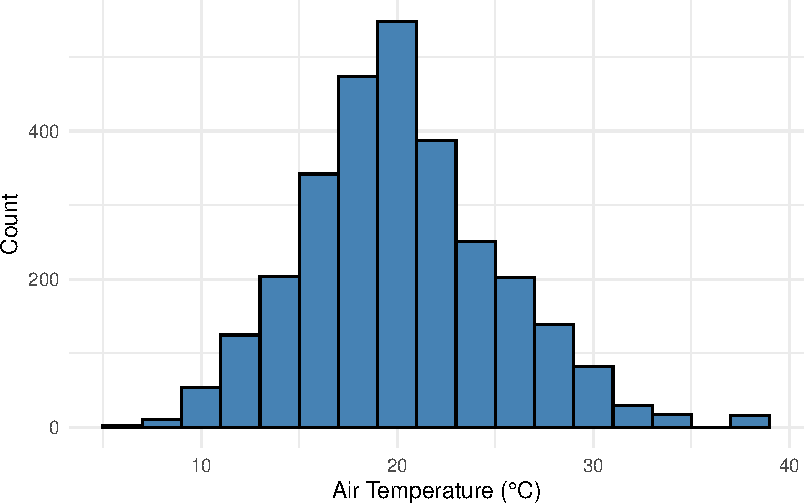
\includegraphics{paper_files/figure-pdf/fig-his1-1.pdf}

}

\caption{\label{fig-his1}Air Temperature Distribution}

\end{figure}%

Wind speed affects both the comfort of beachgoers and water quality.
Figure~\ref{fig-bar1} illustrates the average wind speed at different
Toronto beaches. The x-axis represents the average wind speed in
kilometers per hour (km/h), while the y-axis lists the names of the
beaches. The chart is horizontally oriented for clarity, with the wind
speed values increasing from left to right.The lightblue bars represent
the average wind speed at each beach, and the bars are arranged in
descending order of wind speed. The chart highlights the variability in
wind conditions across different beaches, suggesting that some beaches
are more exposed to wind, potentially affecting people's experiences and
water conditions.

\begin{figure}

\centering{

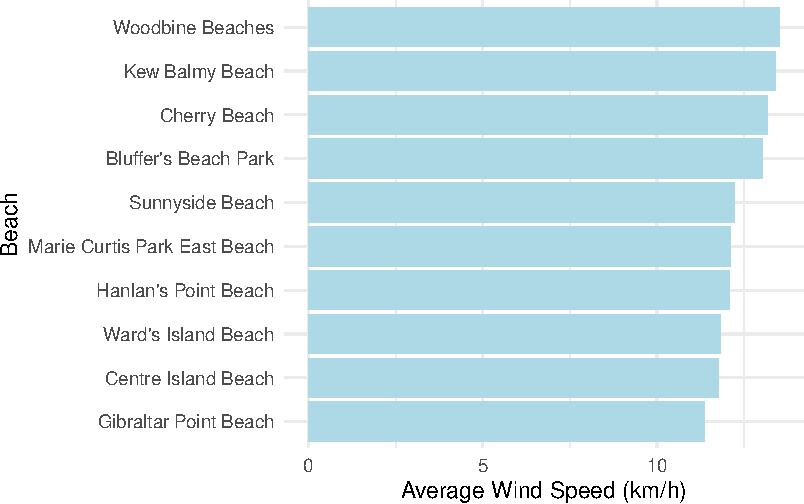
\includegraphics{paper_files/figure-pdf/fig-bar1-1.pdf}

}

\caption{\label{fig-bar1}Average Wind Speed by Beach}

\end{figure}%

Water temperature varies between beaches, which may influence swimmers'
comfort and number of waterfowl in the water. Figure~\ref{fig-bar2}
shows the average water temperature at different Toronto beaches, with
the x-axis representing the average water temperature in degrees Celsius
(°C) and the y-axis listing the beach names. The chart is color-coded to
distinguish each beach, and the bars are arranged in descending order of
average water temperature.

\begin{figure}

\centering{

\centering{

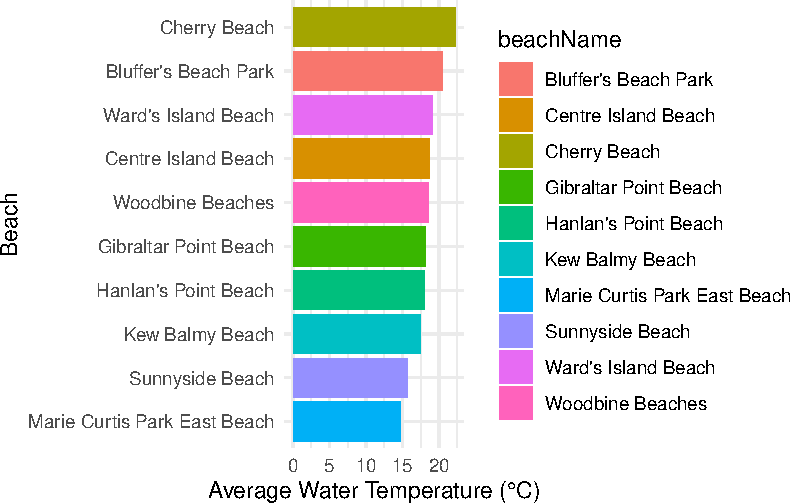
\includegraphics{paper_files/figure-pdf/fig-bar2-1.pdf}

}

\subcaption{\label{fig-bar2}Across different Toronto beaches}

}

\caption{\label{fig-bar2}Average water temperature by beach}

\end{figure}%

Figure~\ref{fig-bar3} shows the total waterfowl count on rainy versus
non-rainy days. The x-axis represents the presence or absence of rain,
with three categories: ``N/A'' (unknown rain status), ``No'' (non-rainy
days), and ``Yes'' (rainy days). The y-axis represents the total number
of waterfowl observed. The chart indicates a noticeable difference in
waterfowl presence based on weather conditions, with more waterfowl
observed on non-rainy days compared to rainy ones. We can see that on
non-rainy days (labeled ``No''), the highest number of waterfowl were
observed, with a count exceeding 60,000. On rainy days (labeled
``Yes''), the total waterfowl count is significantly lower, around
40,000. The ``N/A'' category, representing days with unknown rain
status, shows very few waterfowl, with a total count close to zero.

\begin{figure}

\centering{

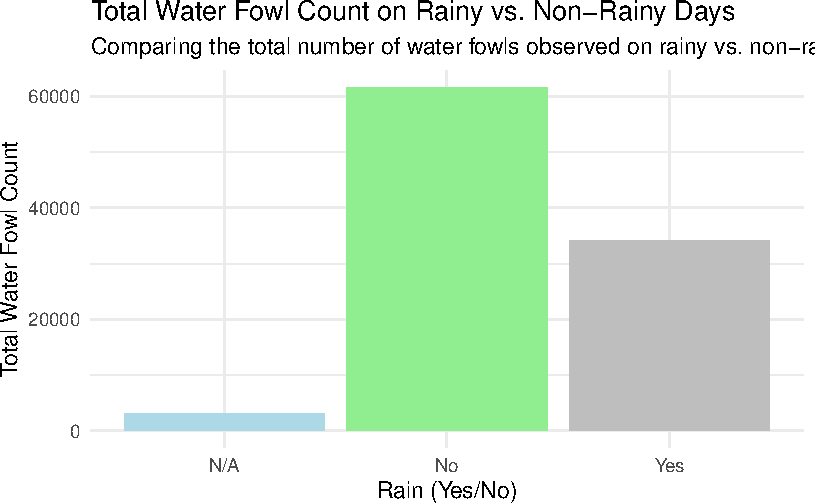
\includegraphics{paper_files/figure-pdf/fig-bar3-1.pdf}

}

\caption{\label{fig-bar3}Total water fowl count on rainy vs non-rainy
days}

\end{figure}%

Figure~\ref{fig-scatter1} illustrates the relationship between wind
speed (x-axis, measured in km/h) and turbidity (y-axis, measured in
NTU). Each point represents an observation, with wind speed along the
horizontal axis and turbidity along the vertical axis. This scatter plot
shows that there is no strong linear relationship between wind speed and
turbidity. However, lower wind speeds tend to be associated with a wide
range of turbidity levels, whereas higher wind speeds appear to be less
common and do not show higher turbidity levels. Most data points are
clustered in areas with lower wind speeds (below 20 km/h) and turbidity
levels below 50 NTU. Some outliers show higher turbidity levels above
150 NTU, especially at lower wind speeds. At wind speeds above 20 km/h,
the data points become scattered, with very few data points over 40
km/h.

\begin{figure}

\centering{

\centering{

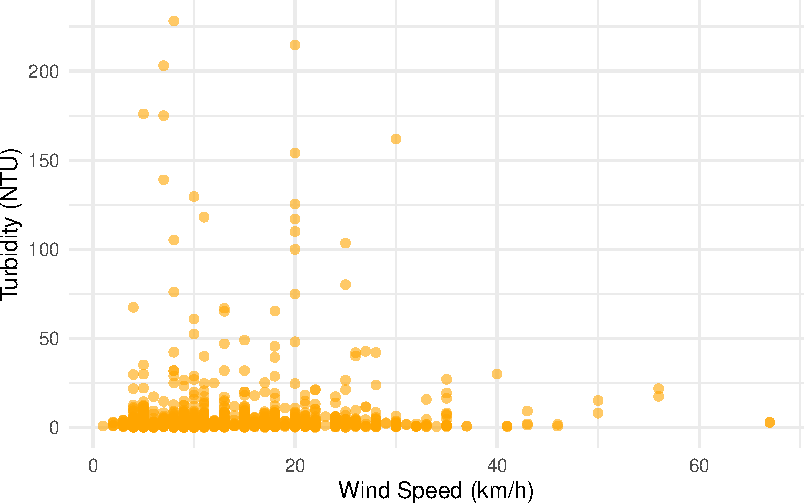
\includegraphics{paper_files/figure-pdf/fig-scatter1-1.pdf}

}

\subcaption{\label{fig-scatter1}Analyzing the relationship between wind
speed and water turbidity}

}

\caption{\label{fig-scatter1}Wind speed vs turbidity}

\end{figure}%

Rainfall significantly impacts water turbidity, as rain can introduce
pollutants and sediments into the water. Figure~\ref{fig-box1} shows the
distribution of turbidity levels (measured in NTU) on rainy versus
non-rainy days. The x-axis represents whether rain was present
(``Yes''), absent (``No''), or unknown (``N/A''), while the y-axis
represents turbidity levels. The box plot suggests that most
observations, whether rainy or not, tend to have lower turbidity levels.
Non-rainy days exhibit a slightly broader spread of turbidity levels,
but the majority of observations have relatively low turbidity (close to
0 NTU), with several outliers reaching beyond 200 NTU. Turbidity levels
were also mostly low in Rainy (Yes) and N/A(Unknown), but there were
outliers over 150 NTU.

\begin{figure}

\centering{

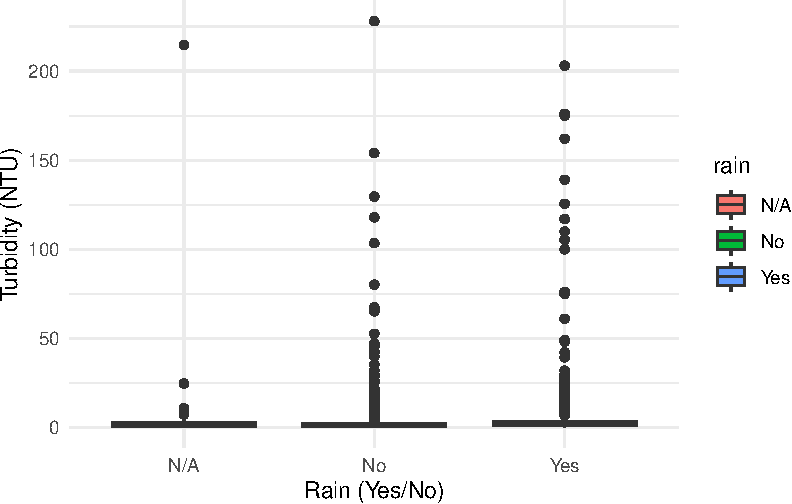
\includegraphics{paper_files/figure-pdf/fig-box1-1.pdf}

}

\caption{\label{fig-box1}Turbidity Levels on Rainy vs.~Non-Rainy Days}

\end{figure}%

\newpage

\section{Discussion}\label{third}

\subsection{}\label{section}

\newpage

\section{Appendix}\label{appendix-a}

\subsection{Variable description}\label{appendix-a.1}

\begingroup\fontsize{10}{12}\selectfont

\begin{longtable}[t]{ll}

\caption{\label{tbl-sum2}}

\tabularnewline

\toprule
Column & Description\\
\midrule
\_id & Unique row identifier for
Open Data database\\
dataCollectionDate & Date observations were
collected\\
beachName & Name of beach where
observations were
collected\\
windSpeed & Wind speed measured in
km/h\\
windDirection & Wind directions - East,
North-East, North,
North-West, West,
South-West, South,
South-E\\
\addlinespace
airTemp & Air temperature in
degrees Celsius\\
rain & Presence of rain - Yes,
No\\
rainAmount & Amount of rainfall in mm
in the last 24 hours\\
waterTemp & Water temperature in
degrees Celsius\\
waterFowl & Count of water fowl seen\\
\addlinespace
waveAction & Observations on wave
action - high, low,
moderate, none\\
waterClarity & Visual state of water's
clarity - free form text\\
turbidity & Turbidity of water
measured in Nephelometric
Turbidity Units (NTUs)\\
\bottomrule

\end{longtable}

\endgroup{}

Description of variables in the dataset

\newpage

\section*{References}\label{references}
\addcontentsline{toc}{section}{References}

\phantomsection\label{refs}
\begin{CSLReferences}{1}{0}
\bibitem[\citeproctext]{ref-opendatatoronto}
Gelfand, Sharla. 2022. \emph{Opendatatoronto: Access the City of Toronto
Open Data Portal}.
\url{https://CRAN.R-project.org/package=opendatatoronto}.

\bibitem[\citeproctext]{ref-citeR}
R Core Team. 2023. \emph{R: A Language and Environment for Statistical
Computing}. Vienna, Austria: R Foundation for Statistical Computing.
\url{https://www.R-project.org/}.

\bibitem[\citeproctext]{ref-saleem2022validation}
Saleem, Faizan, Thomas A Edge, and Herb E Schellhorn. 2022.
{``Validation of qPCR Method for Enterococci Quantification at Toronto
Beaches: Application for Rapid Recreational Water Monitoring.''}
\emph{Journal of Great Lakes Research} 48 (3): 707--16.

\bibitem[\citeproctext]{ref-saleem2023same}
Saleem, Faizan, Herb E Schellhorn, Albert Simhon, and Thomas A Edge.
2023. {``Same-Day Enterococcus qPCR Results of Recreational Water
Quality at Two Toronto Beaches Provide Added Public Health Protection
and Reduced Beach Days Lost.''} \emph{Canadian Journal of Public Health}
114 (4): 676--87.

\bibitem[\citeproctext]{ref-sanchez2021region}
Sanchez, Johanna, Jordan Tustin, Cole Heasley, Mahesh Patel, Jeremy
Kelly, Anthony Habjan, Ryan Waterhouse, and Ian Young. 2021.
{``Region-Specific Associations Between Environmental Factors and
Escherichia Coli in Freshwater Beaches in Toronto and Niagara Region,
Canada.''} \emph{International Journal of Environmental Research and
Public Health} 18 (23): 12841.

\bibitem[\citeproctext]{ref-rohan}
Wickham, Hadley, Mara Averick, Jennifer Bryan, Winston Chang, Lucy
D'Agostino McGowan, Romain François, Garrett Grolemund, et al. 2019a.
{``Welcome to the {tidyverse}.''} \emph{Journal of Open Source Software}
4 (43): 1686. \url{https://doi.org/10.21105/joss.01686}.

\bibitem[\citeproctext]{ref-tidyverse}
---------, et al. 2019b. {``Welcome to the {tidyverse}.''} \emph{Journal
of Open Source Software} 4 (43): 1686.
\url{https://doi.org/10.21105/joss.01686}.

\bibitem[\citeproctext]{ref-dplyr}
Wickham, Hadley, Romain François, Lionel Henry, Kirill Müller, and Davis
Vaughan. 2023. \emph{Dplyr: A Grammar of Data Manipulation}.
\url{https://CRAN.R-project.org/package=dplyr}.

\bibitem[\citeproctext]{ref-young2023recreational}
Young, Ian, J Johanna Sanchez, Binyam Negussie Desta, Cole Heasley, and
Jordan Tustin. 2023. {``Recreational Water Exposures and Illness
Outcomes at a Freshwater Beach in Toronto, Canada: A Prospective Cohort
Pilot Study.''} \emph{PLoS One} 18 (6): e0286584.

\bibitem[\citeproctext]{ref-kableExtra}
Zhu, Hao. 2024. \emph{kableExtra: Construct Complex Table with 'Kable'
and Pipe Syntax}. \url{https://CRAN.R-project.org/package=kableExtra}.

\end{CSLReferences}




\end{document}
